%%% template.tex
%%%
%%% This LaTeX source document can be used as the basis for your technical
%%% paper or abstract. Regardless of the length of your document, the commands
%%% are all the same.
%%% 
%%% The "\documentclass" command is the first command in your file. If you want to 
%%% prepare a version of your article with line numbers - a "review" version - 
%%% include the "review" parameter:
%%%    \documentclass[review]{acmsiggraph}
%%%

\documentclass[review]{acmsiggraph}

\usepackage{amsmath,amssymb}
\usepackage{algorithm}
\usepackage{algpseudocode}

\newcommand{\cm}{\mathcal{M}}
\newcommand{\by}{\mathbf{y}}
\newcommand{\bx}{\mathbf{x}}
\newcommand{\bt}{\mathbf{t}}
\newcommand{\bc}{\mathbf{c}}
\newcommand{\bs}{\mathbf{s}}
\newcommand{\bp}{\mathbf{p}}
\newcommand{\bq}{\mathbf{q}}
\newcommand{\Cfree}{\mathcal{C}_{\mathrm{free}}}
\newcommand{\Cobs}{\mathcal{C}_{\mathrm{obs}}}
\newcommand{\co}{\mathcal{O}}

%%% Title of your article or abstract.

\title{This Is The Title of My Document}

\author{Stephen N. Spencer\thanks{e-mail:spencer@cs.washington.edu}\\Chair, ACM SIGGRAPH Publications Committee}
\pdfauthor{Stephen N. Spencer}

%%% Used by the ``review'' variation; the online ID will be printed on 
%%% every page of the content.

\TOGonlineid{45678}

% User-generated keywords.

\keywords{radiosity, global illumination, constant time}

%%% The next five lines define the rights management block on the first page.
%%% Replace them with the LaTeX commands provided when the form has been completed.

\CopyrightYear{2016}
\setcopyright{acmcopyright}
\conferenceinfo{CONFERENCE PROGRAM NAME}{MONTH, DAY, and YEAR} 
\isbn{THIS-IS-A-SAMPLE-ISBN}\acmPrice{\$15.00}
\doi{http://doi.acm.org/THIS/IS/A/SAMPLE/DOI}

%%% Start of the document.

\begin{document}

%%% This is the ``teaser'' command, which puts an figure, centered, below 
%%% the title and author information, and above the body of the content.

 \teaser{
   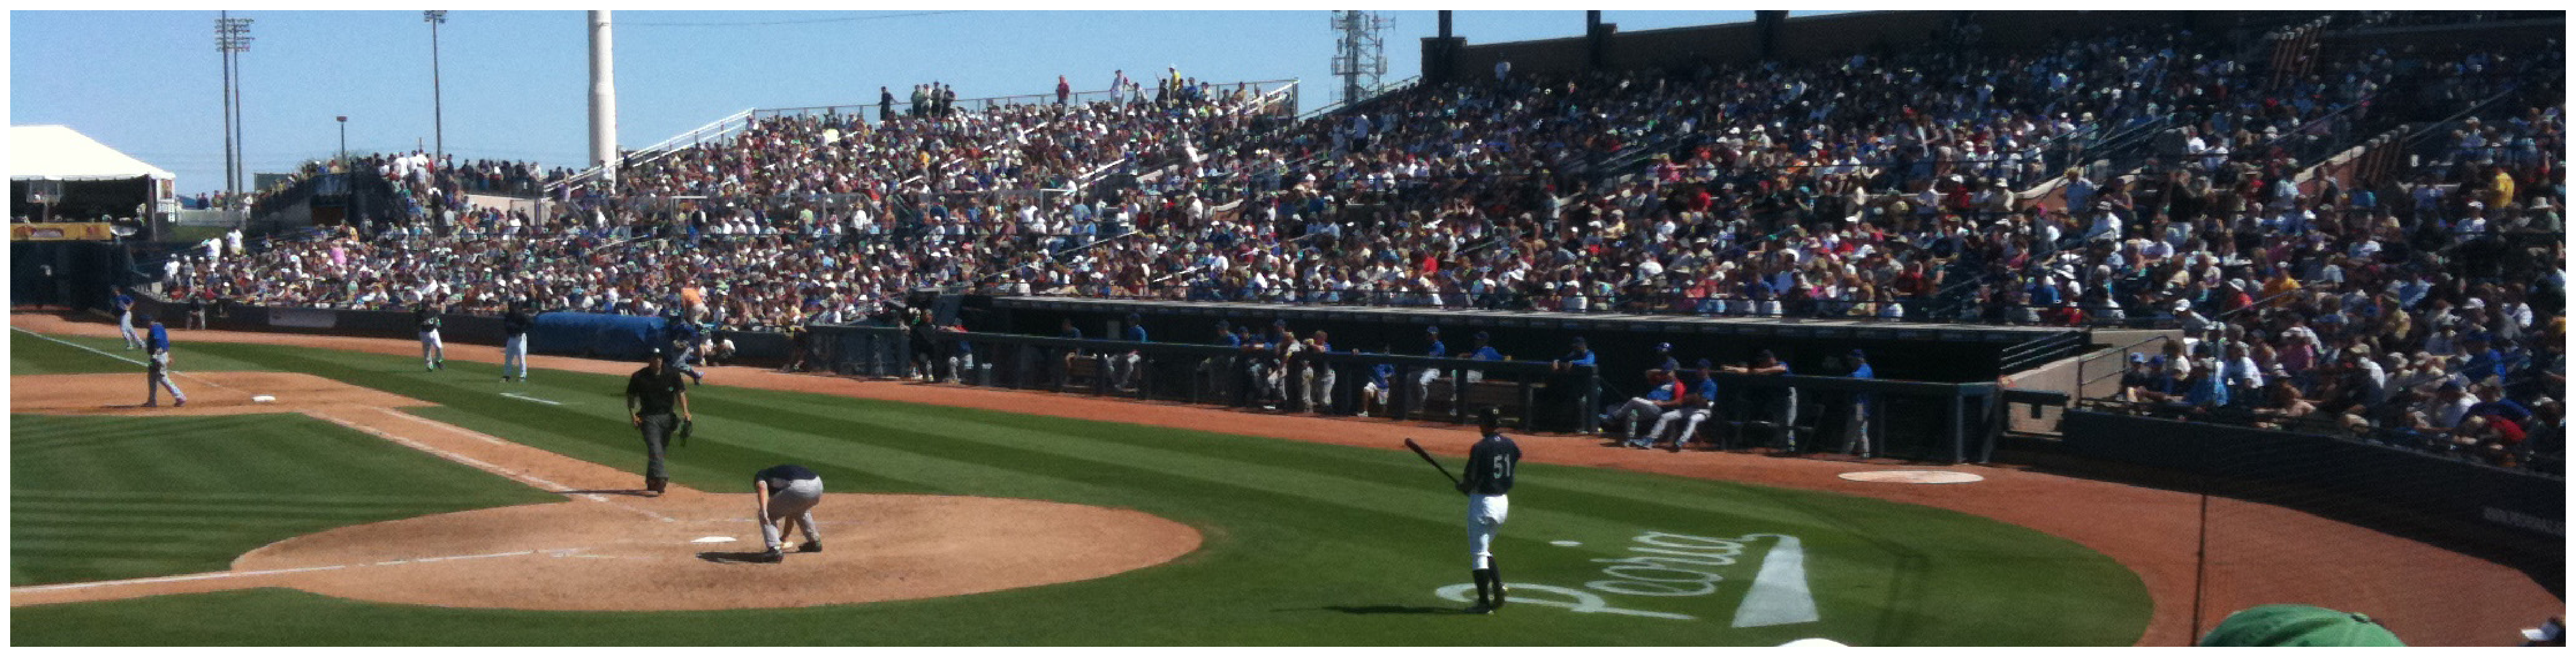
\includegraphics[height=1.5in]{images/sampleteaser}
   \caption{Spring Training 2009, Peoria, AZ.}
 }

\maketitle

\begin{abstract}

\end{abstract}

%
% The code below should be generated by the tool at
% http://dl.acm.org/ccs.cfm
% Please copy and paste the code instead of the example below. 
%
\begin{CCSXML}
<ccs2012>
<concept>
<concept_id>10010147.10010371.10010382</concept_id>
<concept_desc>Computing methodologies~Image manipulation</concept_desc>
<concept_significance>500</concept_significance>
</concept>
<concept>
<concept_id>10010147.10010371.10010382.10010236</concept_id>
<concept_desc>Computing methodologies~Computational photography</concept_desc>
<concept_significance>300</concept_significance>
</concept>
</ccs2012>
\end{CCSXML}

\ccsdesc[500]{Computing methodologies~Image manipulation}
\ccsdesc[300]{Computing methodologies~Computational photography}

%
% End generated code
%

% The next three commands are required, and insert the user-generated keywords, 
% The CCS concepts list, and the rights management text.
% Please make sure there is a blank line between each of these three commands.

\keywordlist

\conceptlist

\printcopyright

\section{Introduction}

Given two entangled rigid bodies in $\mathbb{R}^3$, we want to find a rigid motion of the bodies that disentangles them. It is enough to keep one object fixed (the \emph{obstacle} $\co$) and consider onlly rigid motions of the second object (the \emph{mover} $\cm$). Let $Q = \mathbb{R}^3 \times SO(3)$ denote the configuration space of the mover: to each point $\bq = (\bt, R)\in Q$ is then associated a \emph{pose} $\cm(\bq)$ of $\cm$, with
$$\cm(\bq) = \left\{ \bt + R\bx\ \vert \ \bx \in \cm\right\}.$$
Not all poses are physically possible, since the obstacle gets in the way. Let $\Cobs$ denote the points of configuration that are infeasible because the two objects overlap,
$$\Cobs = \left\{\bq \in Q \ \vert \ \cm(\bq) \cap \co \neq \emptyset\right\},$$
and $\Cfree = Q \setminus \Cobs$ the complementary, feasible space. 

For the purposes of computation, we will restrict our attention to a bounded region $R$ of configuration space, and parameterize the rotational degrees of freedom by Euler angles: $R$ is then a rectangular box in six-dimensional Euclidean space
$$R = [a_x, b_x] \times [a_y, b_y] \times [a_z, b_z] \times [0,2\pi] \times [-\pi,\pi] \times [0, 2\pi]$$
% Note: here we use the Tait-Bryan convention
with the $\phi$ and $\psi$ dimensions periodic. The full configuration space $Q$ extends past $R$ in the $x,y,z$ directions, but we assume that the box is large enough that the entirety of $\Cobs$ lies inside the box. Let $B$ denote the six hyperfaces of $R$ where $x,y$ or $z$ attain their extreme values; given an initial configuration $\bq_0$, the untangling problem can then be formalized as: \textbf{does there exist a path $\gamma$ from $\bq_0$ to $B$, with $\gamma \in \Cfree$?} Here a path is curve in $R$ that is continuous, except for jump discontinuities wherever $\gamma$ ``wraps around'' in the $\phi$ or $\psi$ directions.
\section{Goals}
If it were feasible to explicitly construct a mesh representing $\Cfree$ (or its five-dimensional boundary) the untangling problem would be trivial: a path exists if the connected component (taking into account the periodicity of $R$) of $\Cfree$ containing $\bq_0$ abuts any part of $B$. If a path exists, it can then be reconstructed using e.g. a breadth-first search.

The problem is the dimensionality of $\Cfree$. Given $\co$ and $\cm$ represented as triangulated surfaces in $\mathbb{R}^3$, the boundary of the feasible region $\partial \Cobs$ is not piecewise-affine, and while it can be discretized using five-dimensional hyper-simplices, the number of such simplices needed to thoroughly sample $\partial \Cobs$ is intractable for all but the simplest rigid body geometries.

We therefore seek an algorithm that can find $\gamma$, or prove that a $\gamma$ does not exist, \emph{without} reconstructing $\Cfree$ explicitly. This algorithm must succeed even when $\gamma$ passes through narrrow tunnels, as is often the case for rigid body puzzles. To guarantee that the algorithm is robust even in the face of adversial geometry, we inisist that it possesses the following properties:
\begin{itemize}
\item if a path $\gamma$ exists,the algorithm must find it in finite computation;
\item if no path exists, the algorithm must prove this in finite computation.
\end{itemize}
We now describe our proposed algorithm, which satisfies both of these properties. 

\section{Method Overview}
We will construct a $2^6$-tree (the six-dimensional analogue of an octree) on $R$ and adaptively refine it over time. We will assign to each cell of the tree one of three labels:
\begin{itemize}
\item \emph{free}, if we can prove that the entire cell is contained in $\Cfree$;
\item \emph{obstacle}, if we can prove that the entire cell is contained in $\Cobs$ (and so is impassible to $\gamma$);
\item \emph{unknown}, otherwise.
\end{itemize}
A cell might be classified as unknown because it contains parts of both $\Cobs$ and $\Cfree$, or it might in fact be entirely in one region or entirely in the other, but we are not (yet) able to conclusively determine that this is the case.

Our algorithm then rests on the following observation: if $\bq_0$ is contained in a free cell, and the connected free component of that cell abuts any part of $B$, then $\gamma$ exists, regardless of the status of any remaining unknown cells. Similarly, if obstacle cells completely enclose $\bq_0$ (i.e., if the free-or-unknown connected component of cells containing $\bq_0$ does not abut any part of $B$), then no path $\gamma$ is possible. We will thus keep splitting leaf cells of the $2^6$-tree until one of these two conditions is true. Clearly, there is no profit in spitting free or obstacle cells, but unknown cells can be split, so that hopefully some of the resulting children can be classified as either free or obstracle. 

\begin{algorithm}[h!]
%\small
\caption{\tt Untangling Algorithm} \label{alg:unt}
\begin{algorithmic}[1]
\Function{CanUntangle}{start configuration $\bq_0$}
\State $2^6$-tree $O \gets R$
\While {$c \gets$ \Call{CellContaining}{$\bq_0$} is not free}
\State \Call{Split}{$c$}
\EndWhile
\While{true}
\State $S_1 \gets$ \Call{ConnectedComp}{$\bq_0$, free}
\State $S_2 \gets$ \Call{ConnectedComp}{$\bq_0$, free  or unknown}
\If{$S_1 \cap B \neq \emptyset$}
\Return{true}
\ElsIf{$S_2 \cap B = \emptyset$}
\Return{false}
\Else
\State $c \gets$ \Call{PromisingUnknownCell}{$O$}
\State \Call{Split}{$c$}
\EndIf
\EndWhile
\EndFunction
\end{algorithmic}
\end{algorithm}

We start by creating a $2^6$-tree with only a single leaf node, encompassing all of $R$, and classifying it as unknown. For as long as $\bq_0$ is contained in an unknown cell, we split the cell containing $\bq_0$ and insert the $2^6$ child cells into the tree (and classify them). Since $\bq_0$ is in $\Cfree$ and $\Cfree$ is open, a sufficiently small cell around $\bq_0$ is guaranteed to be free, so this initialization terminates after a finite number of cell splits.

We now check for termination, by examining the connected component of free cells containing $\bq_0$, and the larger connected component of free-or-unknown cells, respectively. If neither termination condition holds, there are still too many unknown cells left in $R$ to find $\gamma$, and so we select an unknown cell, split it, and classify its children. We repeat these steps of checking for termination, and choosing and splitting a cell, until the algorithm terminates. Algorithm~\ref{alg:unt} summarizes the overall procedure. Notice that although \textsc{CanUntangle} answers only whether $\gamma$ exists, in the case the path exists it is straightforward to find an actual path using a bread-first search on the free cells of the final $2^6$-tree.

Several details remain: the method for deciding, given a cell in the tree, whether it should be classified as free, obstacle, or unknown; and the heuristic for choosing a new unknown cell to split at each iteration of the algorithm.

\section{Classifying Cells}
Our main tool in determining whether a cell is guaranteed to be free (or guaranteed to be entirely within the obstacle) is to bound the \emph{maximum distance any point} in $\cm$ can move given the size of the cell.

Let the cell's dimensions be $2w_x \times 2w_y \times 2w_z \times 2w_{\phi} \times 2w_{\theta} \times 2w_{\psi}$ and let $\bc = (\bt_c, R_c)$ be the center of the cell. Let $\bp$  be a point on $\cm$. For any point $\bs = (\bt_s, R_s)$ in the cell, we want a bound $D(\bp)$ on the displacement of $\bp$ between the poses $\cm(\bc)$ and $\cm(\bs)$. This displacement is given by
\begin{align*}
\|\bt_c + R_c\bp - \bt_s - R_s\bp\| &\leq \|\bt_c -\bt_s\| + \|R_c\bp - R_s\bp\|\\
&= \|\bt_c - \bt_s\| + \|R_c \bp - R_c R_c^{-1}R_s \bp\|\\
&= \|\bt_c - \bt_s\| + \| \bp - R_c^{-1}R_s \bp\|\\
&\leq \sqrt{w_x^2 + w_y^2+w_z^2} + \| \bp - R_c^{-1}R_s \bp\|\\
%&\leq \sqrt{w_x^2 + w_y^2+w_z^2} + \|\bp\|\| I - R_c^{-1}R_s\|\\
%&\leq \sqrt{w_x^2 + w_y^2+w_z^2} + \|(R_c - R_s)\bp\| \\
%&\leq \sqrt{w_x^2 + w_y^2+w_z^2} + \|\bp\|\|R_c - R_s\| \\
\end{align*}

To bound the second term, we need to decompose $R_c^{-1}R_s$.
Let $R_X(\phi)$, $R_Y(\theta)$, $R_Z(\psi)$ be rotation matrices w.r.t x, y and z axes.
Thus we can decompose $R_c$ into $R_Z(\psi_c)R_Y(\theta_c)R_X(\phi_c)$, where $psi_c$, $theta_c$, $\phi_c$ are the Euler angles of $R_c$.
Similarly we have $R_s=R_Z(\psi_s)R_Y(\theta_s)R_X(\phi_s)$.
Hence,
\emph{FIXME!!: EULER ANGLES ARE NOT VECTORS, THEY DO NOT COMMUTE}
\begin{align*}
	R_c^{-1}R_s &= (R_Z(\psi_c)R_Y(\theta_c)R_X(\phi_c))^{-1}(R_Z(\psi_s)R_Y(\theta_s)R_X(\phi_s)) \\
	&= R_X(-\phi_c)(R_Y(-\theta_c)(R_Z(-\psi_c)R_Z(\psi_s))R_Y(\theta_s))R_X(\phi_s) \\
	&= R_X(-\phi_c)(R_Y(-\theta_c)R_Z(\psi_s-\psi_c)R_Y(\theta_s))R_X(\phi_s) \\
	&= R_Z(\psi_s-\psi_c)R_Y(\theta_s-\theta_c)R_X(\phi_s-\phi_c) \\
	&= R_Z(\bar{\psi})R_Y(\bar{\theta})R_X(\bar{\phi}) \\
\end{align*}
\emph{FIXME!!: WE ONLY NEED TO BOUND THOSE BAR ANGLES}
Therefore
\begin{align*}
	 & \| \bp - R_c^{-1}R_s \bp\| \\
	=& \| \bp - R_Z(\psi_s-\psi_c)R_Y(\theta_s-\theta_c)R_X(\phi_s-\phi_c)\bp\| \\
	\le& \| \bp - R_X(\phi_s-\phi_c)\bp \| \\
	 &+ \| R_X(\phi_s-\phi_c)\bp - R_Y(\theta_s-\theta_c)R_X(\phi_s-\phi_c)\bp \| \\
	 &+ \|R_Y(\theta_s-\theta_c)R_X(\phi_s-\phi_c)\bp \\
	 &  - R_Z(\psi_s-\psi_c)R_Y(\theta_s-\theta_c)R_X(\phi_s-\phi_c)\bp\| \\
	=& \| (I - R_X(\phi_s-\phi_c))\bp \| \\
	 &+ \| (I - R_Y(\theta_s-\theta_c))R_X(\phi_s-\phi_c)\bp \| \\
	 &+ \| (I - R_Z(\psi_s-\psi_c))R_Y(\theta_s-\theta_c)R_X(\phi_s-\phi_c)\bp\| \\
	=& \| 2\sin(\frac{\phi_s-\phi_c}{2})\bp \| \\
	 &+ \| 2\sin(\frac{\theta_s-\theta_c}{2})R_X(\phi_s-\phi_c)\bp \| \\
	 &+ \| 2\sin(\frac{\psi_s-\psi_c}{2})R_Y(\theta_s-\theta_c)R_X(\phi_s-\phi_c)\bp\| \\
	\le& \| 2\sin(w_\phi)\bp \| \\
	 &+ \| 2\sin(w_\theta)R_X(\phi_s-\phi_c)\bp \| \\
	 &+ \| 2\sin(w_\psi)R_Y(\theta_s-\theta_c)R_X(\phi_s-\phi_c)\bp\| \\
	=& 2\|\bp\|(|\sin(w_\phi)|+|\sin(w_\theta)|+|\sin(w_\psi)|)
\end{align*}
Thus, the upper bound of $\|\bt_c + R_c\bp - \bt_s - R_s\bp\|$ is
\[
\sqrt{w_x^2 + w_y^2+w_z^2} + 2\|\bp\|(|\sin(w_\phi)|+|\sin(w_\theta)|+|\sin(w_\psi)|)
\]

% TODO: We need a figure here

Now that we have $D$, we can use it to classify the cell. Suppose that $\bc \in \Cfree$, so that the cell is either a free cell, or an unknown cell. We compute the \emph{closest distance} $D_c$ between $\co$ and $\cm(\bc)$:
$$D_c = \min_{\bx \in \co} \min_{\by \in \cm(\bc)} \|\bx-\by\|.$$
Now we compare $D$ and $D_c$. If $D < D_c$, then no matter what pose $\cm$ takes within the cell, the points on $\cm$ cannot move a large enough distance to reach any part of $\co$, and so the cell must lie entirely in $\Cfree$. Otherwise, the cell's status is unknown.

Similarly, if $\bc \in \Cobs$, its status can be classified as obstacle or unknown by comparing $D$ to the \emph{penetration depth}
$$D_p = \max_{\bx \in \cm(\bc)} \min_{\by \in \mathbb{R}^3\setminus \co} \|\bx - \by\|.$$
If $D < D_p$, the cell is guaranteed to be an obstacle cell. Otherwise, its status is unknown.
\section*{Acknowledgements}

\bibliographystyle{acmsiggraph}
\bibliography{template}
\end{document}

% vim: tw=0
